%%%%%%%%%---Packages and document settings---%%%%%%%%%
\documentclass[twoside,twocolumn]{article}

  \usepackage{blindtext}      % Package to generate dummy text throughout this template 
  
  \usepackage[sc]{mathpazo}   % Use the Palatino font
  \linespread{1.05}           % Line spacing - Palatino needs more space between lines
  \usepackage[T1]{fontenc}    % Use 8-bit encoding that has 256 glyphs
  \usepackage{microtype}      % Slightly tweak font spacing for aesthetics
  
  \usepackage[spanish]{babel} % Language hyphenation and typographical rules
  \usepackage[utf8]{inputenc} % para poder utilizar acentos sin que te jodan
  
  \usepackage[hmarginratio=1:1,top=32mm,columnsep=20pt]{geometry}     % Document margins
  \usepackage[hang, small,labelfont=bf,up,textfont=it,up]{caption}    % Custom captions under/above floats in tables or figures
  \usepackage{booktabs}       % Horizontal rules in tables
  
  \usepackage{lettrine}       % The lettrine is the first enlarged letter at the beginning of the text
  
  \usepackage{enumitem}       % Customized lists
  \setlist[itemize]{noitemsep}  % Make itemize lists more compact
  
  \usepackage{abstract}       % Allows abstract customization
  \renewcommand{\abstractnamefont}{\normalfont\bfseries}      % Set the "Abstract" text to bold
  \renewcommand{\abstracttextfont}{\normalfont\small\itshape} % Set the abstract itself to small italic text
  
  \usepackage{titlesec}                                   % Allows customization of titles
  \renewcommand\thesection{\Roman{section}}               % Roman numerals for the sections
  \renewcommand\thesubsection{\roman{subsection}}         % roman numerals for subsections
  \renewcommand\thesubsubsection{\arabic{subsubsection}}   % roman numerals for subsections
  \titleformat{\section}[block]{\Large\scshape\centering}{\thesection.}{1em}{}    % Change the look of the section titles
  \titleformat{\subsection}[block]{\large}{\thesubsection.}{1em}{}                % Change the look of the section titles
  \titleformat{\subsubsection}[block]{\it}{\quad\footnotesize\thesubsubsection.}{0.5em}{}                % Change the look of the section titles
  %\titleformat{\paragraph}[block]{\it}{\quad\footnotesize:}{0.1em}{}                % Change the look of the section titles

  \usepackage{fancyhdr}     % Headers and footers
  \pagestyle{fancy}         % All pages have headers and footers
  \fancyhead{}              % Blank out the default header
  %\fancyfoot{}              % Blank out the default footer
  \fancyhead[C]{Detección de partículas con CMOS $\bullet$ Mayo 2018 $\bullet$ D. F. Balmaceda}   % Custom header text
  %\fancyfoot[RO,LE]{\thepage} % Custom footer text
  
  \usepackage{titling}      % Customizing the title section
  
  \usepackage{hyperref}     % For hyperlinks in the PDF
  \usepackage{graphics}     % standard graphics specifications
  \usepackage{graphicx}     % alternative graphics specifications
  \usepackage{longtable}    % helps with long table options
  \usepackage{svg}          % para gráficos .svg
  \usepackage[binary-units=true]{siunitx}      % para las unidades
  \usepackage{datetime}


%%%%%%%%%---Title, authors, date & abstract---%%%%%%%%%
\title{Análisis de interacciones de partículas mediante implementación de una librería para su detección con sensores CMOS}
  \author{%
    \textsc{Darío Federico Balmaceda} \\[1ex]     %  Your name
    \normalsize Laboratorio Detección de Partículas y Radiación. Centro Atómico Bariloche \\                                    %  Your institution
    \normalsize \href{mailto:leschatten@gmail.com}{\texttt{leschatten@gmail.com}}                   %  Your email address
    %\and                                                                      %  Uncomment if 2 authors are require
    %\textsc{Jane Smith} \\[1ex]                  % duplicate these 4 lines
    %\normalsize University of Utah \\ % Second author's institution           % if more
    %\normalsize \href{mailto:jane@smith.com}{jane@smith.com}
  }
  \date{\today}                                                                % Leave empty to omit a date
  \renewcommand{\maketitlehookd}{
    \begin{abstract}
      \noindent
      Lorem ipsum dolor sit amet, consectetuer adipiscing elit. Etiam lobortis facilisis sem. Nullam nec mi et
        nequepharetra sollicitudin. Praesent imperdiet mi nec ante. Donec ullamcorper, felis non sodales commodo,
        lectusvelit ultrices augue, a dignissim nibh lectus placerat pede. Vivamus nunc nunc, molestie ut, ultricies
        vel,semper in, velit. Ut porttitor. Praesent in sapien. Lorem ipsum dolor sit amet, consectetuer adipiscing
        elit.Duis fringilla tristique neque. Sed interdum libero ut metus. Pellentesque placerat. Nam rutrum augue
        aleo. Morbi sed elit sit amet ante lobortis sollicitudin. Praesent blandit blandit mauris. Praesent lectus
        tellus,aliquet aliquam, luctus a, egestas a, turpis. Mauris lacinia lorem sit amet ipsum. Nunc quis urna
        dictumturpis accumsan semper
      %TODO: ABSTRACT
    \end{abstract}
  }

  \setlength{\droptitle}{-4\baselineskip}                 % Move the title up
  \pretitle{\begin{center}\Large\bfseries}                 % Article title formatting
  \posttitle{\end{center}}                                % Article title closing formatting

%
  %%%%%%%%%%%%%%%%%%%%%%%%%%%%%%%%%%%%%%%%%%
  %%%%                                 %%%%%
  %%%%  And now, begin the document... %%%%%
  %%%%                                 %%%%%
  %%%%%%%%%%%%%%%%%%%%%%%%%%%%%%%%%%%%%%%%%%
\begin{document}
  
  \maketitle              % Print the title
  
  %%%%%%%%%%%%%%%%%%%%%%%%%%%%%%%%%%%%%%%%%%%%%%%%%%%
  \section{Introducción}
    %\cite{Lane}
    \lettrine[nindent=0em,lines=3]{L} orem ipsum dolor sit amet, consectetur adipiscing elit.
      Etiam lobortis facilisis sem. Nullam nec mi et nequepharetra sollicitudin.
      Praesent imperdiet mi nec ante. Donec ullamcorper, felis non sodales commodo,
      lectusvelit ultrices augue, a dignissim nibh lectus placerat pede.
    %TODO: reemplazar esto

    \subsection{Sensores CMOS-APS}
      Un sensor de píxeles activos (APS por sus siglas en inglés) es un sensor que detecta la radiación basado en tecnología CMOS.
      Este tipo de sensores son ampliamente utilizados de manera comercial debido a su
      bajo costo de producción y sus buenos resultados en fotografía.
      Estos sensores están presentes en teléfonos celulares, ordenadores portatiles, cámaras de acción,
      y en la mayoría de los dispositivos electrónicos que posee una cámara.

      Los sensores consisten en un arreglo matricial de fotodiodos, 
      que producen una corriente eléctrica que varía en función de la intensidad de luz recibida.
      Por cada fotodiodo, se incorpora un amplificador y un conversor analógico digital (ADC) para la lectura de los datos.

    \subsubsection{Filtro de Bayer}

      Típicamente los sensores CMOS destinados para fotografías poseen un filtro de Bayer, 
      el mismo consiste en un arreglo de filtros rojos, verdes y azules dispuestos como se muestra en la Fig.~\ref{fig:bayer}.
      De esta forma, cada píxelposee la información de un único rango de longitudes de onda, 
      esto permite una composición de la imagen en 3 colores diferentes, de manera análoga al ojo humano.

      \begin{figure}[h]
        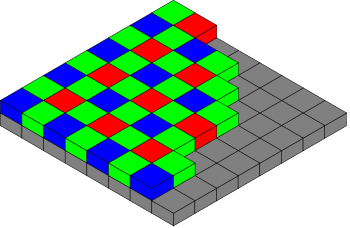
\includegraphics[width=0.35\textwidth]{figures/Bayer_pattern.png}
        \caption{Filtro de Bayer típico de un sensor CMOS-APS. Por cada 4 píxeles 2 son verdes, 1 es rojo y 1 es azul.
          El color verde es utilizado dos veces debido a la sensibilidad al verde del ojo humano.}
        \label{fig:bayer}
      \end{figure}

    \subsection{Interacción de la radiación de partículas con la materia}
      

    \subsection{Rayos cósmicos}
      Los rayos cósmicos son partículas que llegan desde el espacio y bombardean constantemente la Tierra desde todas direcciones.
      La mayoría de estas partículas son protones o núcleos de átomos.
      Al interactuar con la atmósfera terrestre, estas partículas generan una cascada de muónes %TODO: escribir esto un poco mejor


    \subsection{Picos $K_{\alpha}$ y $K_{\beta}$}

  %%%%%%%%%%%%%%%%%%%%%%%%%%%%%%%%%%%%%%%%%%%%%%%%%%%
  \section{Configuración experimental}\label{sec:conf_exp}

    \subsection{Sensor CMOS}\label{sec:conf_exp:CMOS}
      Se ha utilizado el sensor OmniVision OV5647 de la cámara Raspicam V1.3 cuyo precio ronda los 23 dólares.
      El sensor posee una resolución de	$2592$x$1944$ píxeles, lo que le una resolución total de $5$ MP.
      El tamaño de un píxel de \SI{1.4}{\micro\meter} x \SI{1.4}{\micro\meter}.
      El capacidad de carga máxima hasta llegar a saturación es de $4300$ electrones (\emph{Well Capacity}).
      El sensor posee un ADC de 10 bits por píxel.
      El tamaño total por imagen raw de unos \SI{6.4}{\mega\byte}

      Debido a que cada píxel presenta una electrónica separada, se tomó una foto.
    %TODO: además poner todos los resultados anteriores que me pertimiteron entender cómo funciona todo

    \subsection{Raspberry}
      Se utilizó una Raspberry Pi modelo B, con una memoria micro SD de \SI{16}{\giga\byte}, para la obtención de imágenes.
      Debido a la resolución de las imágenes, la profundidad de bits de la imagenes y del tamaño del sistema operativo \emph{Raspbian}, 
      la memoria disponible
      permitió almacenar del orden de 1000 fotografías en simultáneo.

    %TODO: Para un informe por ahí es conveniente poner los detalles de la raspistill y la librería en python
    \subsection{Librería raspiraw}
      Para la adquisicón de datos se utilizó la librería {\it raspiraw}\cite{raspiraw} debido a la rapidez con la que se toman los datos.
      En el apéndice~\ref{sec:ap_alternatives} se muestran otras alternativas que son más lentas para la toma de datos,
      pero que pueden resultar más simples y sencillas de implementar.

      Los datos sin procesamiento (datos \emph{raw}) eran guardados con extensión raw.
      Los mismos consistian en $1952$ filas de 3264~bytes.
      Las últimas $8$ filas de dato no contienen información y no son utilizadas,
      ya que sólo existen debido a que $1952$ es menor múltiplo de $16$     % FIXME: Y por qué 16!?
      mayor a las $1944$ que posee el sensor filas del sensor (ver sección \ref{sec:conf_exp:CMOS}.

      De la misma forma, los último $24$~bits de cada fila no son utilizados y deben ser descartados.
      % FIXME: Encontrar por qué deben ser descartados

      Cada píxel se representa mediante un número de $10$~bits (ver sección \ref{sec:conf_exp:CMOS}),
      En una misma columna, los píxeles son agrupados de a $4$, formando una estructura de $5$~bytes.
      En los primeros $4$~bytes se encuentran los bits más significativos de los 4 píxeles que conforman la estructura.
      El quinto byte contiene los últimos $2$~bits menos significativos de cada píxel.
      La manera en la que los bits están ordenados en un grupo se muestra en la Fig.~\ref{fig:arreglo}

      \begin{figure}[h]
        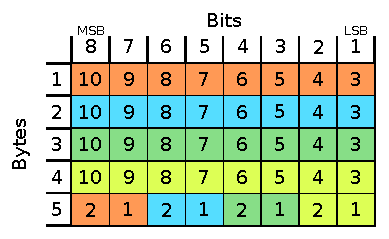
\includegraphics[width=0.47\textwidth]{figures/bayer_bytes.pdf}
        \caption[LoF entry]{Representación de un grupo 4 píxeles.

        Los $40$~bits de los $4$ píxeles están distribuídos como ilustra la figura.
        Colores distintos corresponden a píxeles distintos.

        En las filas se indica en número de byte (siendo $5$ en total).

        En cada celda se encuentra un número que representa el bit de información de un píxel,
        siendo 1 el bit menos signficativo (LSB) y 10 el bit más signficativo (MSB).}
        \label{fig:arreglo}
      \end{figure}

      Los parámetros que permite variar esta librería son:
      \paragraph{Tiempo de exposición}
        Se define como el tiempo en el que sensor acumula carga.
        A mayor tiempo de exposición, mayor es la carga leída por el detector.
        
        En lo que sigue, se utilizó un tiempo de exposición de \SI{0.5}{\milli\second}, a no ser que se aclare lo contrario.

      \paragraph{Cuadros por segundos}
        También conocido como \emph{fps} por sus siglas en inglés.
        Se refiere a la frecuencia con la que se toman las imágenes y generalmente viene expresado en fotografías por segundo.
        
        En lo que sigue, se capturó a 2 cuadros por segundo,a no ser que se aclare lo contrario.

      %\paragraph{Ganancia}

    \subsection{Emisor de rayos X}
      Para la calibración de la carga dada por el detector CMOS como función de la energía se utilizó un emisor de rayos Xavier
      %TODO: Explicar un poco cómo funciona y decir que es de Cu.
  
    \subsection{Observación de rayos cósmicos.}
      Utilizando la librería es posible idenficar eventos en simultaneidad con la toma de fotos,
      por lo que se implementó un sistema que guarde solamente las imágenes que poseen pixeles que superen un umbral establecido.
      Debido al ruido de fondo, dicho umbral se ajustó en $75$ Unidades de ADC.

      Como se verá en la sección \ref{sec:}
  
  %%%%%%%%%%%%%%%%%%%%%%%%%%%%%%%%%%%%%%%%%%%%%%%%%%% 
  \section{Resultados}\label{sec:results}
    Para probar el correcto funcionamiento de la librería, se utilizó el poder de procesamiento en dos aplicaciones diferentes.
    Una de ellas consistió en detectar Rayos Cósmicos, y la otra la de observar los picos $K_{\alpha}$ y $K_{\beta}$ de diferentes elementos.

    \subsection{Determinación del ruido de fondo}\label{sec:results:background}
      Se tomaron 30 imágenes con tiempo con tiempo de exposición de \SI{0.5}{\milli\second} a 2 cuadros por segundos (\emph{fps}).
      Se promediaron las 30 imágenes para obtener una estimación sobre el ruido de fondo con la configuración dada. 
      En la Fig.~\ref{fig:background} se muestra el promedio por píxel de las fotografías tomadas.

      \begin{figure}[h]
        
\includegraphics[width=0.47\textwidth]{figures/06-04-18_09-27-42.eps} % TODO: cambiar por background.png
        \caption{Promedio de las 30 imagenes.
          En la misma se observa una dependencia del valor promedio como función de la posición.
          Esta dependencia es más sensible como función de la columna del píxel. }
        \label{fig:background}
      \end{figure}
      %FIXME: La foto de background.png está mal hecha, la nueva foto se encuentra en la carpeta results.

    \subsection{Mediciones de picos $K_{\alpha}$ y $K_{\beta}$ y calibración de energía}\label{sec:results:peaks}
      Se analizó el espectro de Cu, Fe y Ca utilizando la librería \emph{ParticleDetections}.
      Para esto se realizó un histograma de la carga de los eventos.
      En estos espectros fue posible identificar los picos $K_{\alpha}$ y $K_{\beta}$ de Cu y los picos $K_{\alpha}$ del Fe y del Ca,
      esta identificación y asociación nos permitió hacer una calibración de energía como función del canal.
      tal como se muestra en la Fig.~\ref{fig:spectrum_x-ray}.
      
    \begin{figure}[h]
      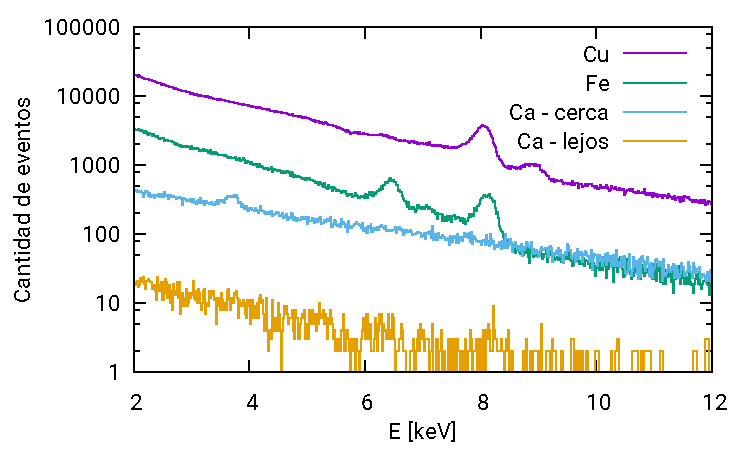
\includegraphics[width=0.47\textwidth]{figures/x-ray_spectrum.pdf}
      \caption{Espectro patronum!}
      \label{fig:spectrum_x-ray}
    \end{figure}

    Conociendo la energía característica de cada uno de estos picos, % TODO: insertar referencia
    se realizó una calibración del valor raw de un pixel como función de la carga (energía) depositada.
    % FIXME: Poner la consideración de que el fotón se frena
    Esta calibración se muestra en la Fig.~\ref{fig:x-ray_calibration}

    \begin{figure}[h]
      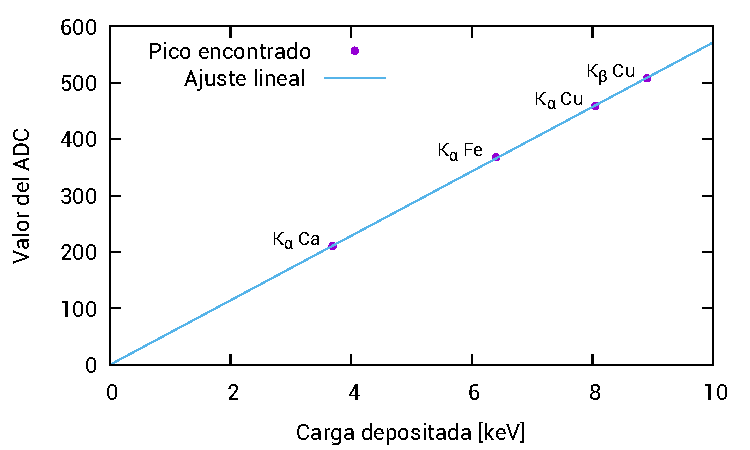
\includegraphics[width=0.47\textwidth]{figures/x-ray_calibration} %FIXME: Poner el valor de la pendiente
      \caption{Calibración del canal del sensor como función de la energía de los picos $K_{\alpha}$ y $K_{\beta}$ encontrados.
        En el mismo se puede apreciar que la relación es lineal y la relación carga por unidad de ADC obtenida es de $ $ %FIXME: Poner valor
      }
      \label{fig:x-ray_calibration}
    \end{figure}

    \subsection{Medición de Rayos Cósmicos}\label{sec:results:cosmic_ray}


    \begin{figure}[h]
      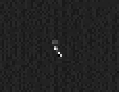
\includegraphics[width=0.47\textwidth]{figures/06-04-18_09-27-42.pdf} % TODO: Poner los pixeles :(
      \caption{Recorte de una imagen tomada en la que se observa un evento.}
      \label{fig:cosmic_ray}
    \end{figure}

    Debido a la baja estadística que se presenta sobre los rayos cósmicos no resulta viable calcular la frecuencia
    con la que estos eventos suceden.


  %%%%%%%%%%%%%%%%%%%%%%%%%%%%%%%%%%%%%%%%%%%%%%%%%%%
  \section{Conclusiones}


  %%%%%%%%%%%%%%%%%%%%%%%%%%%%%%%%%%%%%%%%%%%%%%%%%%% 
  \bibliographystyle{siam}
  \bibliography{bibliography}

  %%%%%%%%%%%%%%%%%%%%%%%%%%%%%%%%%%%%%%%%%%%%%%%%%%%
  \section*{Agradecimientos}
    Se agradece la colaboración de Xavier Bertou por la experiencia brindada y por
    acompañar el trabajo en forma constante.

    A Miguel Sofo por la disponibilidad y por su flexibilidad a la hora de trabajar.
    % TODO: decidir, más gente?
    % TODO: Agregar a alguien que Bertou me dijo pero me colgué
   
  %%%%%%%%%%%%%%%%%%%%%%%%%%%%%%%%%%%%%%%%%%%%%%%%%%%
  \clearpage
  \appendix
  \section{Alternativas a Raspiraw}\label{sec:ap_alternatives}
  
  \subsection{Raspistill y Raspivid}
    Ambos vienen por defectos instalados en el sistema operativo \emph{Raspbian}.
    Raspistill permite capturar fotografías en formato \emph{Joint Photographic Experts Group} (jpeg/jpg).
    Si bien las imágenes tomadas presentan un post-procesamiento, Rapistill es capaz de añadir a la imagen los datos sin procesar (\emph{raw}),

    Por el otro lado, raspivid permite grabar videos en formato \emph{H.264}.
    Este formato también presenta compresión de datos, al igual que .jpg, pero no existe parámetro que permita obtener las imágenes sin procesamiento.
    Por lo debe ser utilizado de manera ilustrativa y cuantitativa, pero no cuantitativa.

  \subsection{Picamera, librería en Python}
    La librería Picamera presenta en su documentación una forma para obtener los datos \emph{raw}, sin procesamiento previo.
    %TODO: Completar

\end{document}

    



